%!Mode:: "TeX:UTF-8"
\documentclass[a4paper,11pt,UTF8]{ctexart}

\usepackage{indentfirst} %缩进
\usepackage{xeCJK}    %使用系统字体
\usepackage{fancyhdr} %自定义页眉页脚
\pagestyle{empty}                   %不设置页眉页脚
\usepackage{amsmath, amsthm, amssymb, amsfonts} %数学公式
\usepackage[a4paper,left=3cm,right=3cm,top=3cm,bottom=3cm]{geometry}
%\usepackage[tmargin=1in,bmargin=1in,lmargin=1.25in,rmargin=1.25in]{geometry}.
\usepackage{booktabs} %插入表格
\usepackage[section]{placeins} %避免浮动
\usepackage{listings} %插入代码
\usepackage{ctex}     %中文宏包
\usepackage[svgnames, table]{xcolor} %彩色表格
\usepackage{algorithm}          %伪代码
\usepackage{algorithmicx}
\usepackage{algpseudocode}
\usepackage{algorithm,algpseudocode,float}
\usepackage{lipsum}
\usepackage{enumitem}           %调整列举环境
\usepackage{url}
\usepackage{fontspec,xunicode}
\defaultfontfeatures{Mapping=tex-text} %如果没有它,会有一些 tex 特殊字符无法正常使用,比如连字符。
\usepackage{subcaption}
\usepackage{graphicx}
\graphicspath{{imgs/}}

%%%%%%%%%%%%%%%%%%%%%%%%%%%%%%%%%%%%%%%%%%%%%%%%%%%%%%%%%%%%%%%%
% 缩进及行间距
%%%%%%%%%%%%%%%%%%%%%%%%%%%%%%%%%%%%%%%%%%%%%%%%%%%%%%%%%%%%%%%%
\setlength{\parindent}{22pt} %重新定义缩进长度
\setlength{\baselineskip}{20pt}  %定义行间距
%\renewcommand{\baselinestretch}{1.1} %定义行间距

%%%%%%%%%%%%%%%%%%%%%%%%%%%%%%%%%%%%%%%%%%%%%%%%%%%%%%%%%%%%%%%%
% 列表设置
%%%%%%%%%%%%%%%%%%%%%%%%%%%%%%%%%%%%%%%%%%%%%%%%%%%%%%%%%%%%%%%%
\setenumerate{fullwidth,itemindent=\parindent,listparindent=\parindent,itemsep=0ex,partopsep=0pt,parsep=0ex}
\setenumerate[2]{label=\alph*),leftmargin=1.5em}  %二级item设置
\setitemize{itemindent=38pt,leftmargin=0pt,itemsep=-0.4ex,listparindent=26pt,partopsep=0pt,parsep=0.5ex,topsep=-0.25ex}
\setdescription{itemindent=38pt,leftmargin=0pt,itemsep=-0.4ex,listparindent=26pt,partopsep=0pt,parsep=0.5ex,topsep=-0.25ex}

%%%%%%%%%%%%%%%%%%%%%%%%%%%%%%%%%%%%%%%%%%%%%%%%%%%%%%%%%%%%%%%%
% 图的标题行间距设置
%%%%%%%%%%%%%%%%%%%%%%%%%%%%%%%%%%%%%%%%%%%%%%%%%%%%%%%%%%%%%%%%
\newcommand{\bottomcaption}{%
\setlength{\abovecaptionskip}{6pt}%
\setlength{\belowcaptionskip}{6pt}%
\caption}


%%%%%%%%%%%%%%%%%%%%%%%%%%%%%%%%%%%%%%%%%%%%%%%%%%%%%%%%%%%%%%%%
% 字体定义
%%%%%%%%%%%%%%%%%%%%%%%%%%%%%%%%%%%%%%%%%%%%%%%%%%%%%%%%%%%%%%%%
\setmainfont{Times New Roman}  %默认英文字体.serif是有衬线字体sans serif无衬线字体
\setmonofont{Consolas}
\setCJKmainfont[ItalicFont={楷体}, BoldFont={黑体}]{宋体}%衬线字体 缺省中文字体为
\setCJKsansfont{黑体}
\punctstyle{hangmobanjiao}
%-----------------------xeCJK下设置中文字体------------------------------%
\setCJKfamilyfont{song}{SimSun}                             %宋体 song
\newcommand{\song}{\CJKfamily{song}}
\setCJKfamilyfont{fs}{FangSong}                      %仿宋  fs
\newcommand{\fs}{\CJKfamily{fs}}
\setCJKfamilyfont{ktgb}{KaiTi}                      %楷体2312 ktgb
\newcommand{\ktgb}{\CJKfamily{ktgb}}
\setCJKfamilyfont{yh}{Microsoft YaHei}                    %微软雅黑 yh
\newcommand{\yh}{\CJKfamily{yh}}
\setCJKfamilyfont{hei}{SimHei}                              %黑体  hei
\newcommand{\hei}{\CJKfamily{hei}}
\setCJKfamilyfont{hwxk}{STXingkai}                                %华文行楷  hwxk
\newcommand{\hwxk}{\CJKfamily{hwxk}}
%------------------------------设置字体大小------------------------%
\newcommand{\shiyanbaogao}{\fontsize{36pt}{\baselineskip}\selectfont}
\newcommand{\chuhao}{\fontsize{42pt}{\baselineskip}\selectfont}     %初号
\newcommand{\xiaochuhao}{\fontsize{36pt}{\baselineskip}\selectfont} %小初号
\newcommand{\yihao}{\fontsize{28pt}{\baselineskip}\selectfont}      %一号
\newcommand{\erhao}{\fontsize{21pt}{\baselineskip}\selectfont}      %二号
\newcommand{\xiaoerhao}{\fontsize{18pt}{\baselineskip}\selectfont}  %小二号
\newcommand{\sanhao}{\fontsize{15.75pt}{\baselineskip}\selectfont}  %三号
\newcommand{\sihao}{\fontsize{14pt}{\baselineskip}\selectfont}       %四号
\newcommand{\xiaosihao}{\fontsize{12pt}{\baselineskip}\selectfont}  %小四号
\newcommand{\wuhao}{\fontsize{10.5pt}{\baselineskip}\selectfont}    %五号
\newcommand{\xiaowuhao}{\fontsize{9pt}{\baselineskip}\selectfont}   %小五号
\newcommand{\liuhao}{\fontsize{7.875pt}{\baselineskip}\selectfont}  %六号
\newcommand{\qihao}{\fontsize{5.25pt}{\baselineskip}\selectfont}    %七号

%%%%%%%%%%%%%%%%%%%%%%%%%%%%%%%%%%%%%%%%%%%%%%%%%%%%%%%%%%%%%%%%
% 图题字体大小相同
%%%%%%%%%%%%%%%%%%%%%%%%%%%%%%%%%%%%%%%%%%%%%%%%%%%%%%%%%%%%%%%%
\usepackage{caption}
\captionsetup{font={footnotesize}}   % footnotesize = 9pt
\captionsetup[lstlisting]{font={footnotesize}}

%%%%%%%%%%%%%%%%%%%%%%%%%%%%%%%%%%%%%%%%%%%%%%%%%%%%%%%%%%%%%%%%
% 重定义枚举编号为 1),2)...
%%%%%%%%%%%%%%%%%%%%%%%%%%%%%%%%%%%%%%%%%%%%%%%%%%%%%%%%%%%%%%%%
\renewcommand{\labelenumi}{\theenumi}


%%%%%%%%%%%%%%%%%%%%%%%%%%%%%%%%%%%%%%%%%%%%%%%%%%%%%%%%%%%%%%%%
% 重定义section标题
%%%%%%%%%%%%%%%%%%%%%%%%%%%%%%%%%%%%%%%%%%%%%%%%%%%%%%%%%%%%%%%%
\CTEXsetup[format={\sihao\CJKfamily{zhhei}\zihao{4}},number={\chinese{section}},name={,、~},aftername={},indent={0pt},beforeskip={6pt},afterskip={6pt},format+={\flushleft}]{section}
\CTEXsetup[number={\chinese{section}},name={附录, ~~ }]{appendix}



%%%%%%%%%%%%%%%%%%%%%%%%%%%%%%%%%%%%%%%%%%%%%%%%%%%%%%%%%%%%%%%%
% 标题名称中文化
%%%%%%%%%%%%%%%%%%%%%%%%%%%%%%%%%%%%%%%%%%%%%%%%%%%%%%%%%%%%%%%%
\renewcommand\figurename{\hei 图}
\renewcommand\tablename{\hei 表}
\renewcommand\lstlistingname{\hei 代码}
\renewcommand{\algorithmicrequire}{\textbf{输入:}}
\renewcommand{\algorithmicensure}{\textbf{输出:}}
\newtheorem{define}{定义}

%%%%%%%%%%%%%%%%%%%%%%%%%%%%%%%%%%%%%%%%%%%%%%%%%%%%%%%%%%%%%%%%
% 代码设置
%%%%%%%%%%%%%%%%%%%%%%%%%%%%%%%%%%%%%%%%%%%%%%%%%%%%%%%%%%%%%%%%
\lstset{
 columns=fixed,
 numbers=left,                                        % 在左侧显示行号
 numberstyle=\tiny\color{gray},                       % 设定行号格式
 frame=single,                                        % 单线背景边框
 breaklines=true,                                     % 设定LaTeX对过长的代码行进行自动换行
 keywordstyle=\color[RGB]{40,40,255},                 % 设定关键字颜色
 numberstyle=\footnotesize\color{darkgray},
 commentstyle=\it\color[RGB]{0,96,96},                % 设置代码注释的格式
 stringstyle=\rmfamily\slshape\color[RGB]{128,0,0},   % 设置字符串格式
 showstringspaces=false,                              % 不显示字符串中的空格
 language=java,                                        % 设置语言
 basicstyle=\linespread{1.0}\xiaowuhao\ttfamily,                      % 字体字号
 %lineskip=10pt,
 %baselinestretch=1,
}

%%%%%%%%%%%%%%%%%%%%%%%%%%%%%%%%%%%%%%%%%%%%%%%%%%%%%%%%%%%%%%%%
% 伪代码分页
%%%%%%%%%%%%%%%%%%%%%%%%%%%%%%%%%%%%%%%%%%%%%%%%%%%%%%%%%%%%%%%%
\makeatletter
\renewcommand{\ALG@name}{算法}
\newenvironment{breakablealgorithm}
  {% \begin{breakablealgorithm}
   \begin{center}
     \refstepcounter{algorithm}% New algorithm
     \hrule height.8pt depth0pt \kern2pt% \@fs@pre for \@fs@ruled
     \renewcommand{\caption}[2][\relax]{% Make a new \caption
       {\raggedright\textbf{\ALG@name~\thealgorithm} ##2\par}%
       \ifx\relax##1\relax % #1 is \relax
         \addcontentsline{loa}{algorithm}{\protect\numberline{\thealgorithm}##2}%
       \else % #1 is not \relax
         \addcontentsline{loa}{algorithm}{\protect\numberline{\thealgorithm}##1}%
       \fi
       \kern2pt\hrule\kern2pt
     }
  }{% \end{breakablealgorithm}
     \kern2pt\hrule\relax% \@fs@post for \@fs@ruled
   \end{center}
  }
\makeatother



\begin{document}
\xiaosihao\song

\begin{titlepage}
\center{\yihao{\hwxk{武汉大学国家网络安全学院}}}
\vspace{6cm}
\center{\shiyanbaogao{\ktgb{密~码~学~实~验~报~告}}}
\vspace{4cm}

\begin{center}
\begin{large}
\begin{tabular}{rc}
\xiaoerhao{\hei{学\qquad 号}}& \hspace{1.7cm}\xiaoerhao{\hei{2021302181156\hspace{1.7cm}}} \\
\cline{2-2}\\
\xiaoerhao{\hei{姓\qquad 名}}& \xiaoerhao{\hei{赵~伯~俣}}\\
\cline{2-2}\\
\xiaoerhao{\hei{实验名称}}& \xiaoerhao{\hei{分组密码工作模式}}\\
\cline{2-2}\\
\xiaoerhao{\hei{指导教师}}& \xiaoerhao{\hei{何琨}}\\
\cline{2-2}
\end{tabular}
\end{large}
\end{center}
\vfill \hfill
\end{titlepage}
\clearpage

% \centerline{\\[10pt]\erhao{\fs{武 ~汉 ~ 大~ 学}}}
% \centerline{\\[10pt]\yihao{\fs{信~息~隐~藏~实~验~报~告}}}

% \leftline{\\[10pt]\sihao{\hei{\hspace{1.5em} 学生姓名:XXX \hfill 学号:XXXX \hfill 指导教师:XXX }}}

% \leftline{\\[10pt]\sihao{\hei{\hspace{1.5em} 实验地点:新珈楼XXX \hfill }}}

% \leftline{\\[10pt]\sihao{\hei{\hspace{1.5em} 实验时间:第X周周X(X-X节) \hfill }}}



\setlength{\parskip}{6pt}  %定义段间距

\section{实验名称: 分组密码工作模式}
\section{实验目的及要求:}
    \subsection{实验目的}
        $(1)$掌握分组密码的基本概念\par
        $(2)$掌握DES、AES、SMS4密码算法\par
        $(3)$了解分组密码DES、AES、SMS4的安全性\par
        $(4)$掌握分组密码常用工作模式及其特点\par
        $(5)$熟悉分组密码的应用\par
    \subsection{实验要求}
        $(1)$掌握分组密码的ECB、CBC、OFB、CFB、CTR等常用工作模式\par
        $(2)$掌握分组密码的短块加密技术\par
        $(3)$熟悉分组密码各工作模式的(数据掩盖、错误传播、效率等)特点\par
        $(4)$利用分组密码工作模式和短块处理技术实现任意长度输入的加密与解密\par
  

\section{实验设备环境及要求:}
    Windows操作系统,python高级语言开发环境
\newpage
\section{实验内容与步骤:}
    \subsection{分组密码的常用工作模式}

        \subsubsection{电码本模式ECB}
            电码本模式是利用分组密码对明文的各个分组进行加密,\par
            其加密公式为:$C_{i}=E(M_{i},K), i=1,2,\dots ,n$\par
            解密公式为:$M_{i}=D(C_{i},K), i=1,2,\dots ,n$\par
            该模式的加解密流程如下图所示
            \begin{figure}[H]
                \centering
                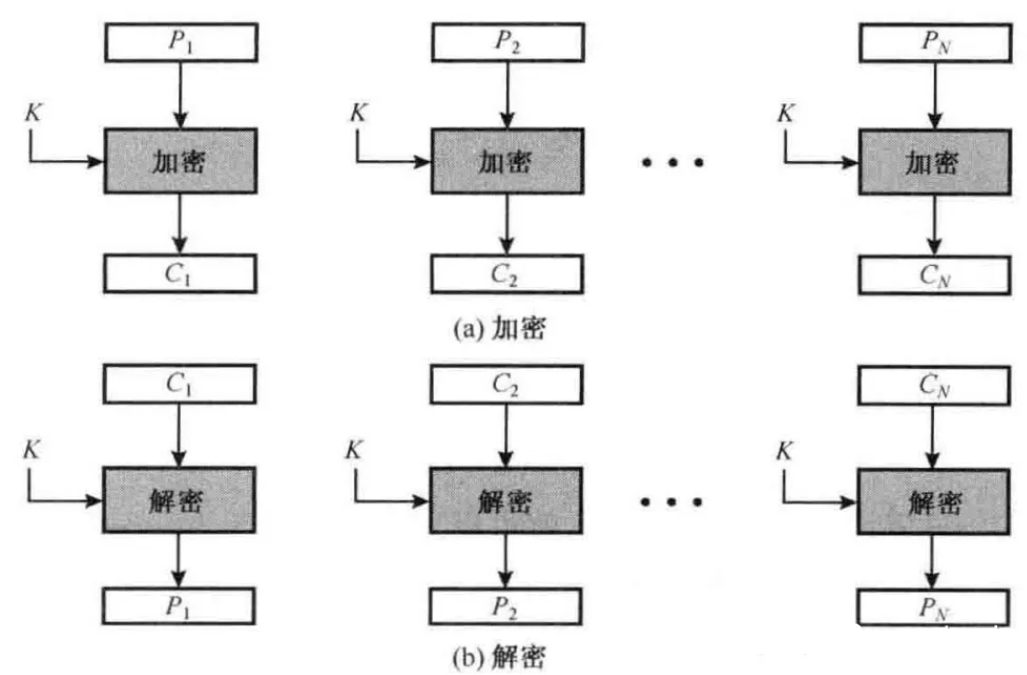
\includegraphics[width=13cm]{ECB.png}
                \bottomcaption{\xiaowuhao{ECB加解密流程}}
            \end{figure}
            在本次实验中的ECB实现代码如下所示
            \lstinputlisting[caption={ECB},captionpos=b]{E:/Python_code/codes/cryptography/lab_3/work_style/ECB/ECB.py}
\newpage
        \subsubsection{密文链接模式CBC}
            密文分组链接模式(Cipher Block Chaining,CBC)中,加密算法的输入是明文分组和前一个密文分组的异或,
            同样均使用相同的密钥进行加密。其中第一个明文加密时,需先与初始向量 异或,再进入加密算法进行加密。\par
            CBC模式的加密公式为:\par
            $C_{i}=\left\{\begin{matrix}E(M_{i}\oplus Z,K),i=1 \\E(M_{i}\oplus C_{i-1},K),i=2,\dots ,n\end{matrix}\right.$\par
            CBC模式解密公式为:\par
            $M_{i}=\left\{\begin{matrix}D(C_{i},K)\oplus Z,i=1 \\D(C_{i},K)\oplus C_{i-1},i=2,\dots ,n\end{matrix}\right. $\par
            加解密过程流程图为:
            \begin{figure}[H]
                \centering
                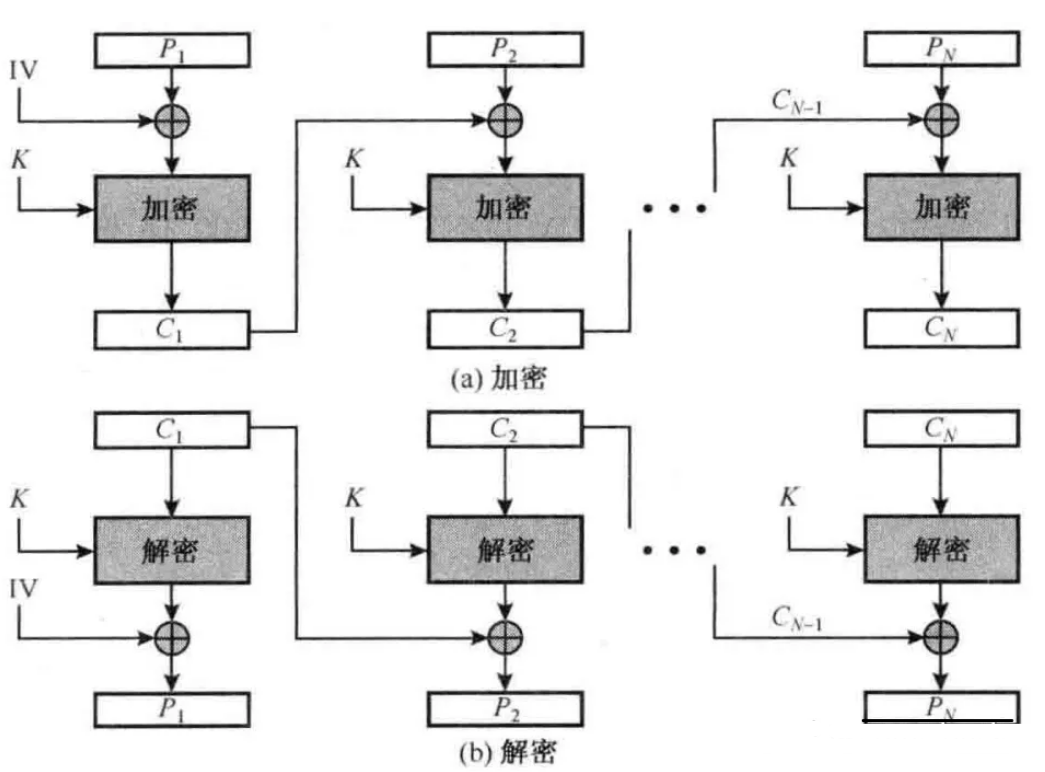
\includegraphics[width=13cm]{CBC.png}
                \bottomcaption{\xiaowuhao{CBC加解密流程}}
            \end{figure}
\newpage
            在本次实验中的CBC实现代码如下所示
            \lstinputlisting[caption={CBC},captionpos=b]{E:/Python_code/codes/cryptography/lab_3/work_style/CBC/CBC.py}
\newpage
        \subsubsection{输出反馈模式OFB}
            输出反馈模式(Output Feedback,OFB)也是一种类似于流密码的工作模式。在这种模式中,明文分组同样没有进入到加密算法中,
            加密算法只是用来计算密钥流的。直接将加密算法的输出反馈到下一分组加密算法的输入中。\par
            其加解密算法流程图为:
            \begin{figure}[H]
                \centering
                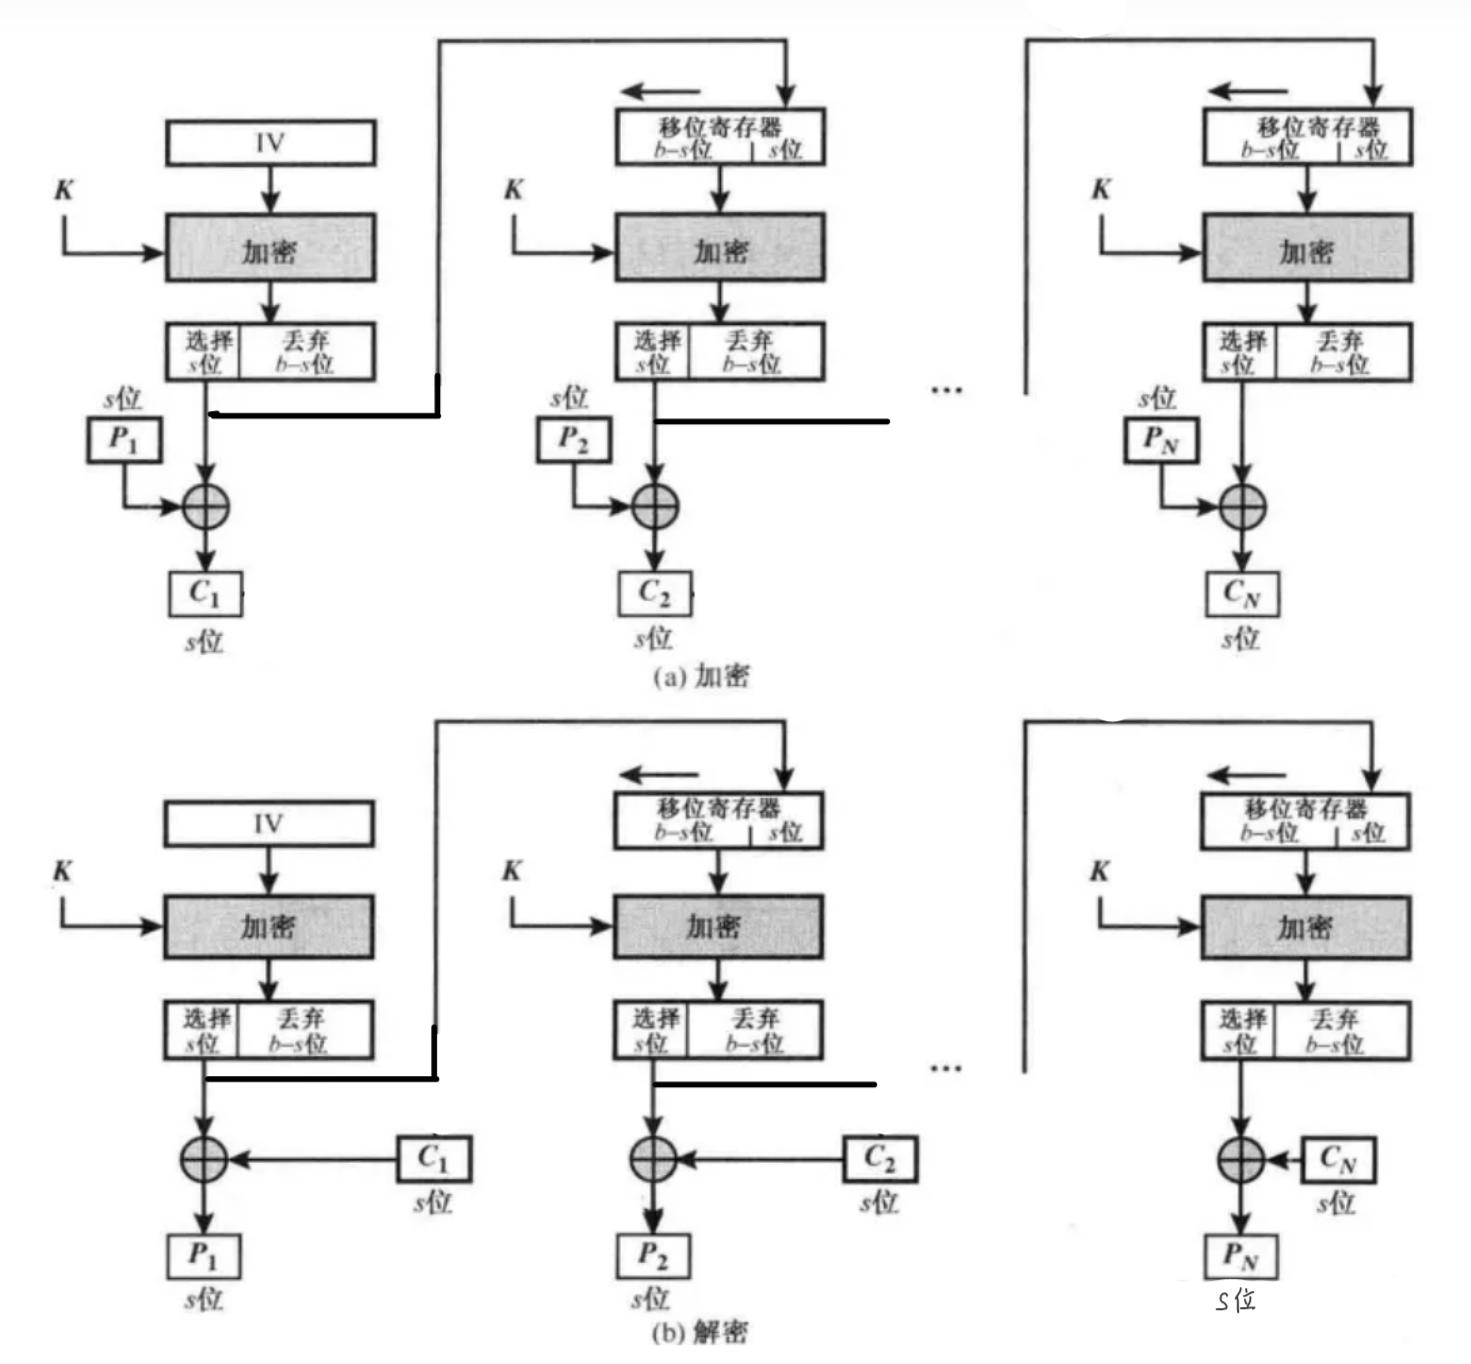
\includegraphics[width=13cm]{OFB.jpg}
                \bottomcaption{\xiaowuhao{OFB加解密流程}}
            \end{figure}
            在本次实验中的OFB实现代码如下所示
            \lstinputlisting[caption={OFB},captionpos=b]{E:/Python_code/codes/cryptography/lab_3/work_style/OFB/OFB.py}

        \subsubsection{密文反馈模式CFB}
            在CFB(Cipher Feedback,CFB)模式下,明文本身并没有进入加密算法中进行加密,而是与加密函数的输出进行了异或,得到了密文。
            其加解密算法流程图为:
            \begin{figure}[H]
                \centering
                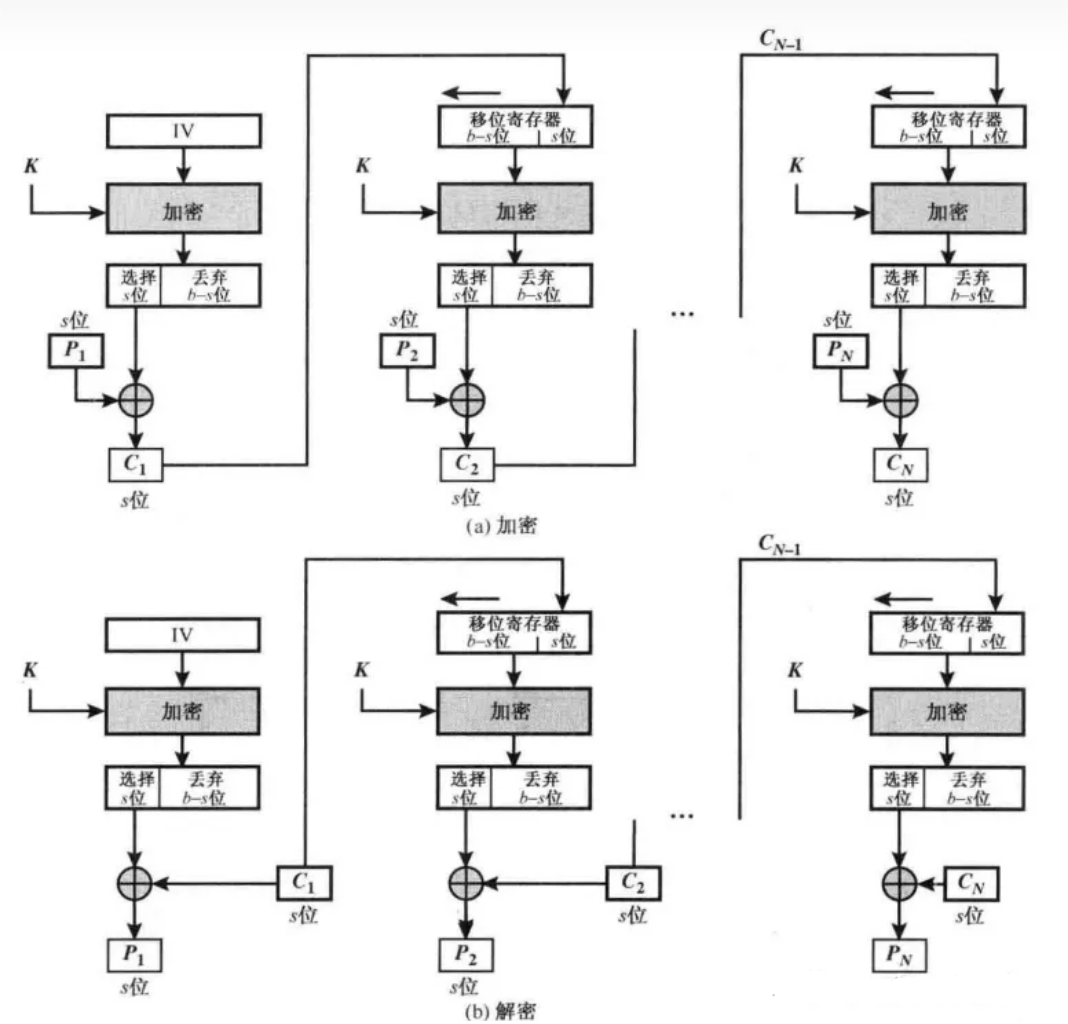
\includegraphics[width=11cm]{CFB.png}
                \bottomcaption{\xiaowuhao{CFB加解密流程}}
            \end{figure}
\newpage
            在本次实验中的CFB的实现代码如下所示
            \lstinputlisting[caption={CFB},captionpos=b]{E:/Python_code/codes/cryptography/lab_3/work_style/CFB/CFB.py}

        \subsubsection{X CBC模式}

            XCBC模式可以处理任意长度的数据,在处理最后一个明文块时,若其不是标准块则需要将其末尾填充字符串‘1’和若干个‘0’
            并且在加密时需要先将填充后的明文块与$C_{i-1}$和$K_{3}$进行异或操作后再进行加密,若最后一个明文块没有进行填充
            则需要将其与$C_{i-1}$和$K_{2}$进行异或操作后再进行加密\par
            XCBC的加密算法公式为:\par
            $C_{i}=\left\{\begin{matrix} E(M_{i}\oplus Z,K_{1}),i=1\\
                 E(M_{i}\oplus C_{i-1},K_{1}),i=2,3,\dots n-1\\
                E(M_{n}\oplus C_{n-1}\oplus K_{2},K_{1}),i=n,and len(M_{n})=32 \\
                E(Pad(M_{n})\oplus C_{n-1}\oplus K_{3},K_{1}),i=n,and len(M_{n})<32
                \end{matrix}\right.$\par
\newpage
            XCBC的解密算法公式为:\par
            $M_{i}=\left\{\begin{matrix} D(C_{i},K_{1})\oplus Z,i=1\\ 
                D(C_{i},K_{1})\oplus C_{i-1},i=2,3,\dots n-1\\
                D(C_{n},K_{1})\oplus C_{n-1}\oplus K_{2},i=n,and len(M_{n})=32 \\
                dePad(D(C_{n},K_{1})\oplus C_{n-1}\oplus K_{3}),i=n,and len(M_{n})<32 \end{matrix}\right.$
            
            XCBC加密算法的流程图如下图所示
            \begin{figure}[H]
                \centering
                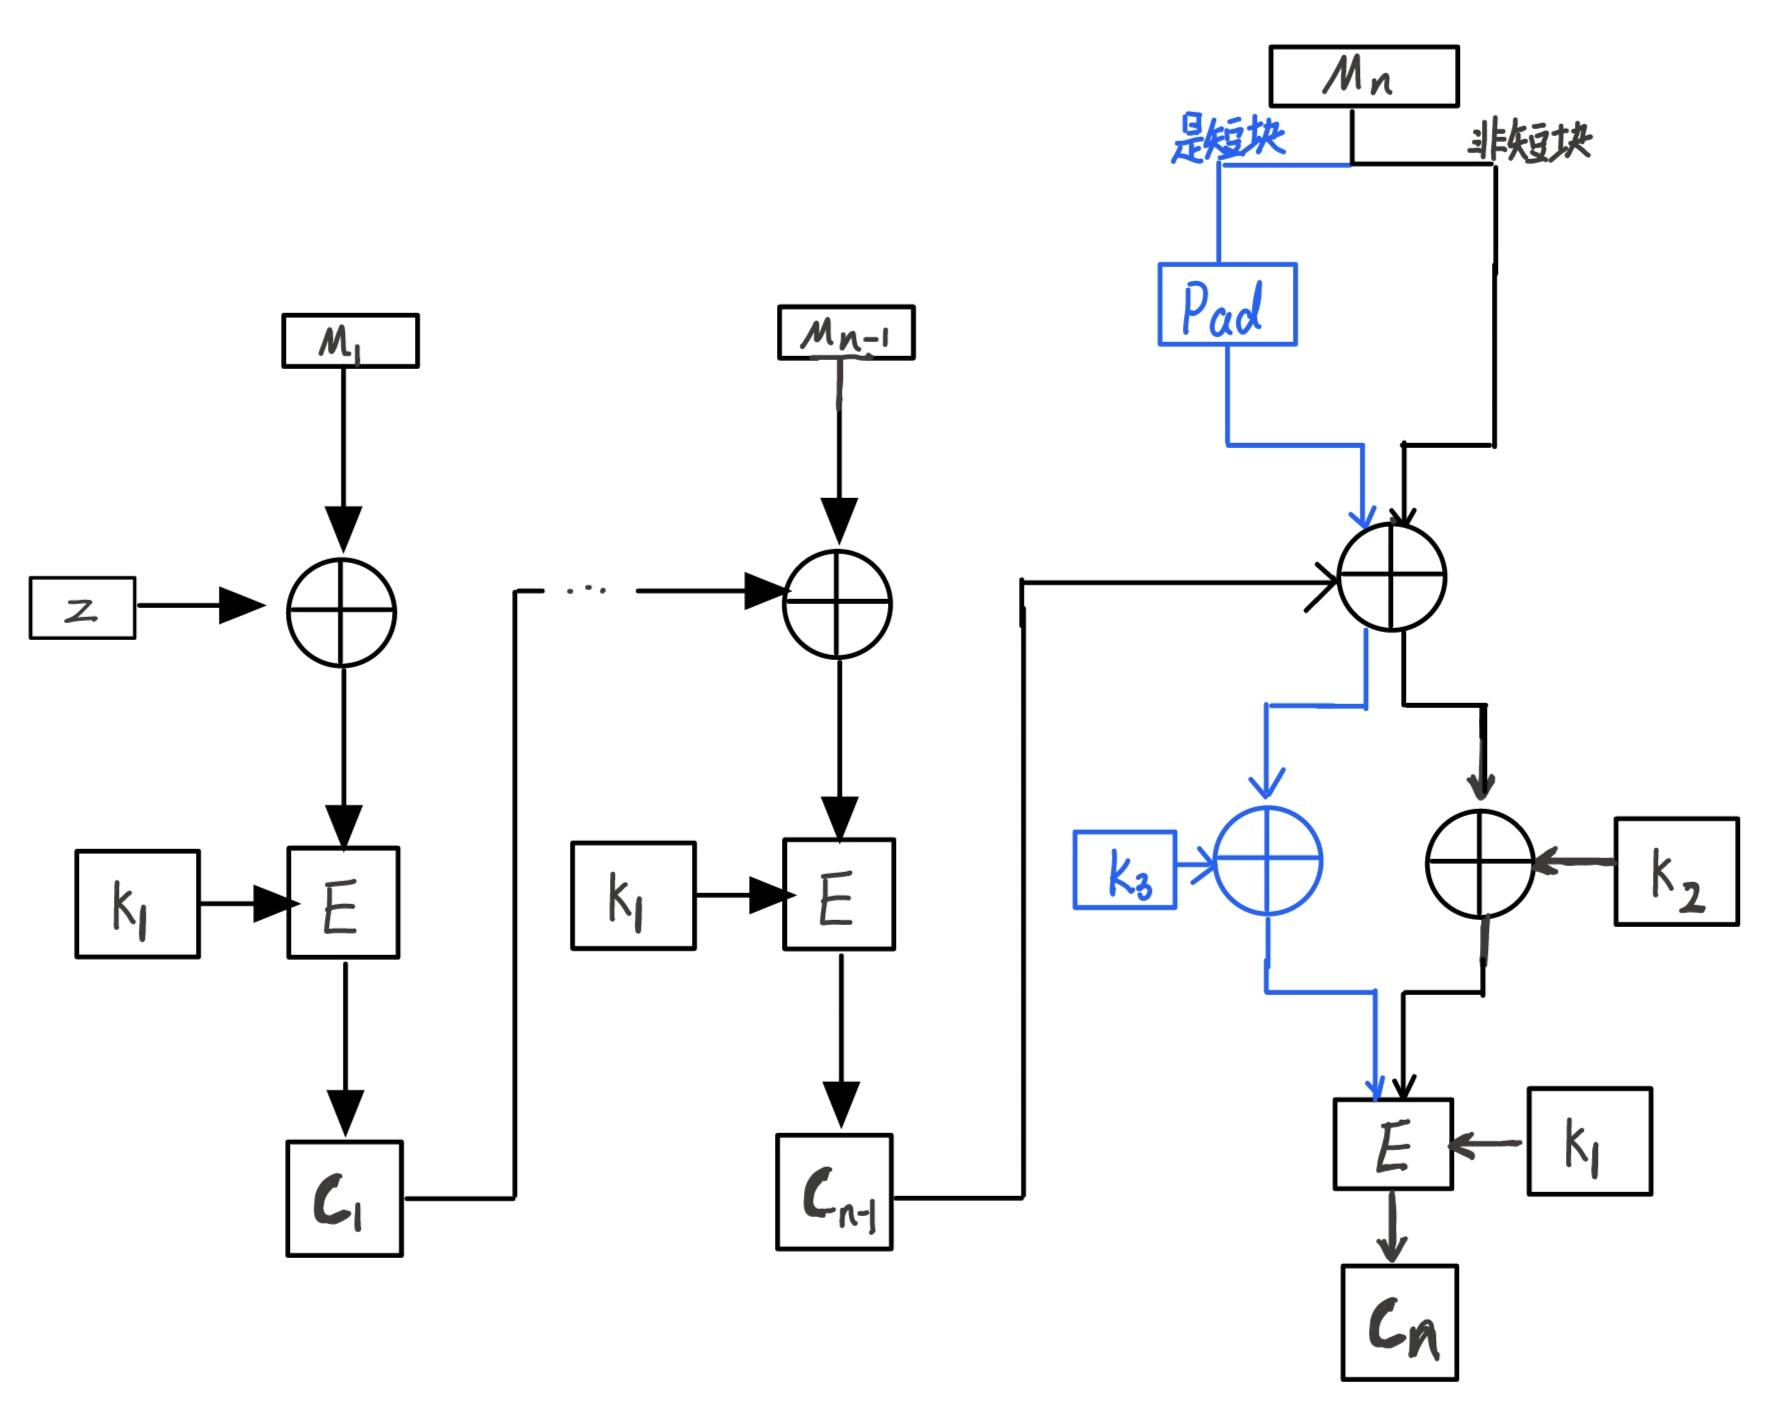
\includegraphics[width=10cm]{XCBC加密.jpg}
                \bottomcaption{\xiaowuhao{XCBC加密流程}}
            \end{figure}
            XCBC解密算法的流程图与加密算法相似,在此不做赘述。\par
            在本次实验中XCBC的实现代码如下所示
            \lstinputlisting[caption={XCBC},captionpos=b]{E:/Python_code/codes/cryptography/lab_3/work_style/XCBC/XCBC.py}

        \subsubsection{计数器模式CTR}
            计数器模式(counter,CTR)也是一种类似于流密码的模式。加密算法只是用来产生密钥流与明文分组异或。区别在于每一次将
            计数器的值进行加一再进行加密操作。
            CTR模式的加密公式为:\par
            $ \left\{\begin{matrix}O_{i}=E(T_{i},K),i=1,2,\dots ,n 
                \\ C_{i}=M_{i}\oplus O_{i},i=1,2,\dots ,n-1\\C_{n}=M_{n}\oplus MSB_{n}(O_{n})\end{matrix}\right.$\par
            CTR模式的解密公式为:\par
            $\left\{\begin{matrix}O_{i}=E(T_{i},K),i=1,2,\dots ,n \\ 
                M_{i}=C_{i}\oplus O_{i},i=1,2,\dots ,n-1\\M_{n}=C_{n}\oplus MSB_{n}(O_{n})\end{matrix}\right.$\par
\newpage
            CTR模式的加密解密算法流程图如下图所示
            \begin{figure}[H]
                \centering
                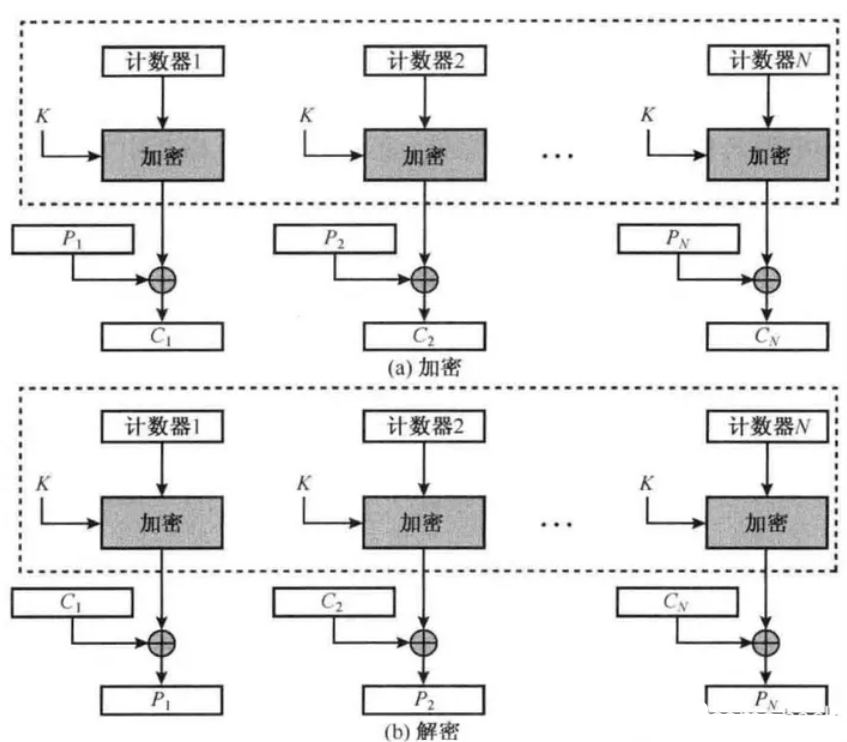
\includegraphics[width=10cm]{CTR.png}
                \bottomcaption{\xiaowuhao{CTR加解密流程}}
            \end{figure}
            在本次实验中CTR的实现代码如下所示
            \lstinputlisting[caption={CTR},captionpos=b]{E:/Python_code/codes/cryptography/lab_3/work_style/CTR/CTR.py}

        \subsubsection{明密文链接模式MCBC}
            明密文链接模式是在CBC的基础上将交付给下一个加密迭代的$C_{n-1}$与明文异或之后再进行之后的操作
            其加密公式为:\par
            $C_{i}=\left\{\begin{matrix} E(M_{i}\oplus Z,K),i=1\\E(M_{i}\oplus M_{i-1}\oplus C_{i-1},K),i=2,3,\dots ,n\end{matrix}\right.$\par
            其解密公式为:\par
            $ M_{i}=\left\{\begin{matrix} D(C_{i},K)\oplus Z,i=1\\D(C_{i},K)\oplus M_{i-1}\oplus C_{i-1},i=2,3,\dots ,n\end{matrix}\right.$\par
            MCBC算法流程图如下图所示
            \begin{figure}[H]
                \centering
                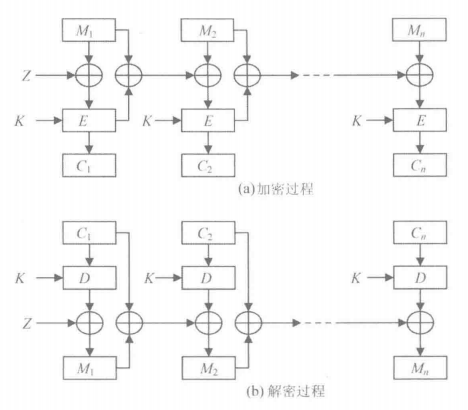
\includegraphics[width=10cm]{MCBC.png}
                \bottomcaption{\xiaowuhao{MCBC加解密流程}}
            \end{figure}
            在本次实验中MCBC的实现代码如下所示
            \lstinputlisting[caption={MCBC},captionpos=b]{E:/Python_code/codes/cryptography/lab_3/work_style/MCBC/MCBC.py}

    \subsection{分组密码的短块处理技术}

        \subsubsection{填充法}
            在本次实验中XCBC工作模式使用填充法来处理短块。主要原理是将短块补充成标准快所需要的长度,
            补充的字符为‘1’以及若干个‘0’在解密时需要将该补充的字符进行消除。
            实现这一步骤的代码如下所示
            \lstinputlisting[caption={填充法实现代码},captionpos=b,firstline=21,lastline=32]{E:/Python_code/codes/cryptography/lab_3/work_style/XCBC/XCBC.py}

        \subsubsection{序列密码加密法}
            序列密码加密法是混合使用分组密码和序列密码两种技术的方案,其中对于标准块用分组密码加密,而对于短块用序列密码加密\par
            序列密码的加密公式为:$C_{n}=M_{n}\oplus MSB_{u}(E(C_{n-1},K))$\par
            序列密码的加解密流程图如下图所示
            \begin{figure}[H]
                \centering
                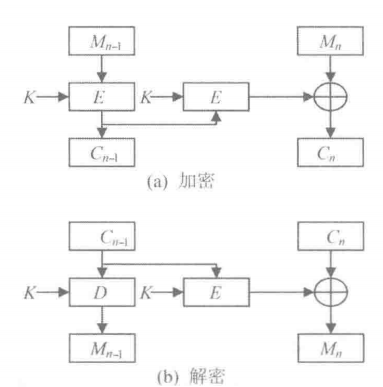
\includegraphics[width=9cm]{序列密码加解密.png}
                \bottomcaption{\xiaowuhao{序列密码加密法}}
            \end{figure}
            在本次实验中实现序列密码加解密的代码如下所示
            \lstinputlisting[caption={序列密码加解密},captionpos=b]{E:/Python_code/codes/cryptography/lab_3/PAD/序列密码/序列密码.py}

        \subsubsection{密文挪用技术}
            密文挪用技术中,在对短块$M_{n}$加密之前,首先从密文$C_{n-1}$中挪出刚好够填充的位数,然后将其填充到$M_{n}$中去
            使得$M_{n}$成为一个标准块,这样$C_{n-1}$却成为了短块,然后再对填充后的$M_{n}$进行加密操作,得到密文$C_{n}$。
            在解密时先对$C_{n}$解密,还原出明文$M_{n}$和从$C_{n-1}$中挪用的数据,把从$C_{n-1}$中所挪用的数据再挪回$C_{n-1}$,
            然后再对$C_{n-1}$解密,还原出$M_{n-1}$。当明文本身就是一个短块时,用初始向量Z代替$C_{n-1}$\par
            密文挪用技术算法流程图如下图所示
            \begin{figure}[H]
                \centering
                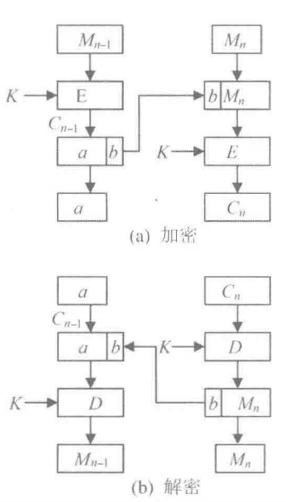
\includegraphics[width=5cm]{密文挪用.png}
                \bottomcaption{\xiaowuhao{密文挪用技术}}
            \end{figure}
            在本次实验中的实现代码如下所示
            \lstinputlisting[caption={密文挪用},captionpos=b]{E:/Python_code/codes/cryptography/lab_3/PAD/密文挪用/密文挪用.py}


    \subsection{各工作模式的特点比较}

        \subsubsection{各工作模式是否能够掩盖明文中的数据模式}
            对于每一种工作模式都选定明文为‘0001000101a198afda78173486153566\\
            0001000101a198afda78173486153566aaa'
            将加密两次得到的结果C1,C2进行比较
            (1)ECB\par
                运行结果如下图所示
                \begin{figure}[H]
                    \centering
                    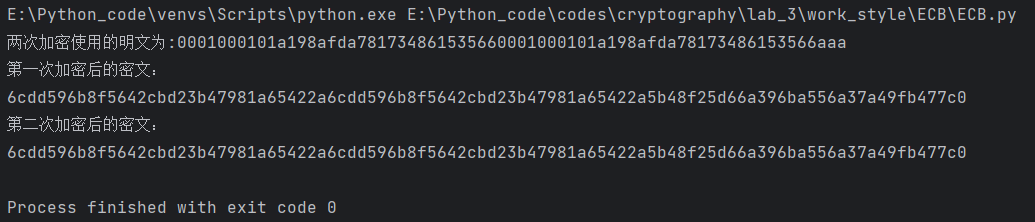
\includegraphics[width=13cm]{ECB_result_1.png}
                    \bottomcaption{\xiaowuhao{ECB相同明文加密两次结果}}
                \end{figure}
                观察结果发现,两次加密得到的结果相同,所以ECB不能够掩盖明文中的数据模式\par

            (2)MCBC\par
            运行结果如下图所示
            \begin{figure}[H]
                \centering
                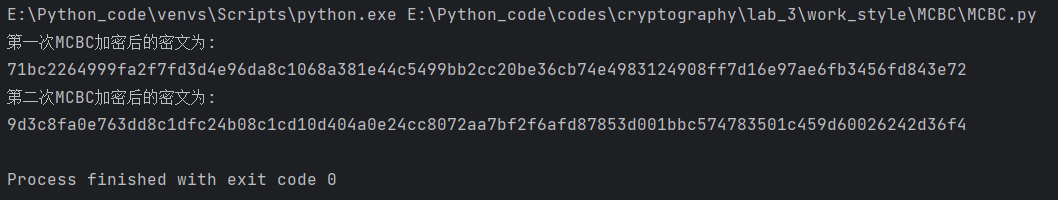
\includegraphics[width=13cm]{MCBC_result_1.png}
                \bottomcaption{\xiaowuhao{MCBC相同明文加密两次结果}}
            \end{figure}
            通过观察发现,两次加密得到的结果不相同,所以MCBC能够掩盖明文中的数据模式\par
\newpage
            (3)CBC\par
                运行结果如下图所示
                \begin{figure}[H]
                    \centering
                    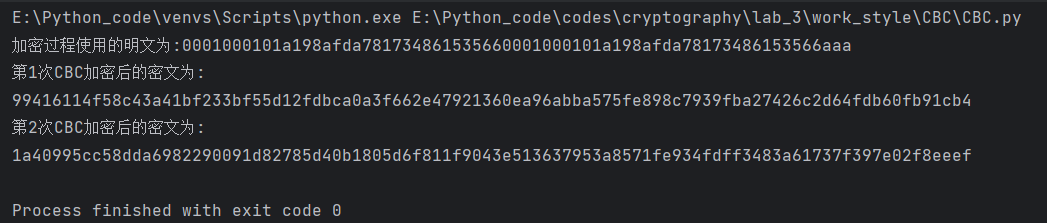
\includegraphics[width=13cm]{CBC_result_1.png}
                    \bottomcaption{\xiaowuhao{CBC相同明文加密两次结果}}
                \end{figure}
                通过观察发现,两次加密得到的结果不相同,所以CBC能够掩盖明文中的数据模式\par

            (4)OFB\par
                运行结果如下图所示
                \begin{figure}[H]
                    \centering
                    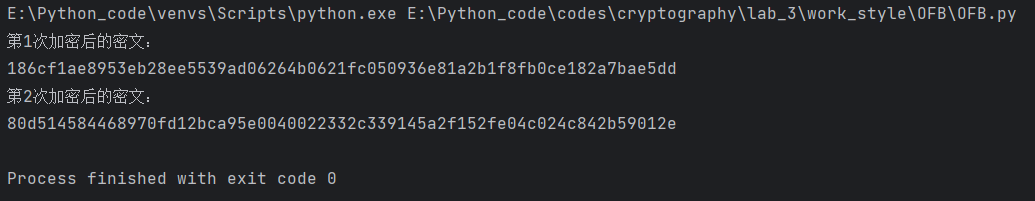
\includegraphics[width=13cm]{OFB_result_1.png}
                    \bottomcaption{\xiaowuhao{OFB相同明文加密两次结果}}
                \end{figure}
                通过观察发现,两次加密得到的结果不相同,所以OFB能够掩盖明文中的数据模式\par

            (5)CFB\par
                运行结果如下图所示
                \begin{figure}[H]
                    \centering
                    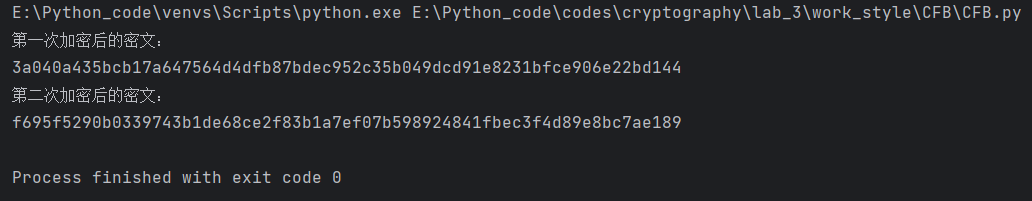
\includegraphics[width=13cm]{CFB_result_1.png}
                    \bottomcaption{\xiaowuhao{CFB相同明文加密两次结果}}
                \end{figure}
                通过观察发现,两次加密得到的结果不相同,所以CFB能够掩盖明文中的数据模式\par
                
            (6)XCBC\par
                运行结果如下图所示
                \begin{figure}[H]
                    \centering
                    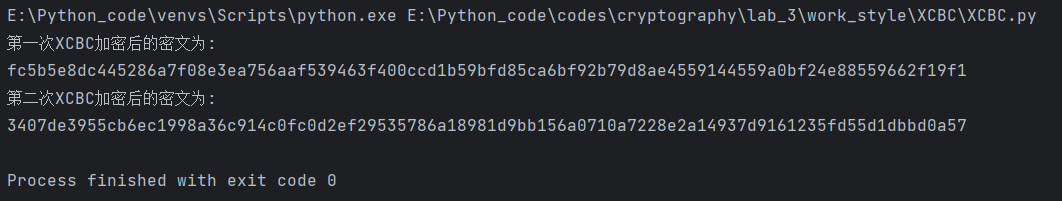
\includegraphics[width=13cm]{XCBC_result_1.png}
                    \bottomcaption{\xiaowuhao{XCBC相同明文加密两次结果}}
                \end{figure}
                通过观察发现,两次加密得到的结果不相同,所以XCBC能够掩盖明文中的数据模式\par

            (7)CTR\par
                运行结果如下图所示
                \begin{figure}[H]
                    \centering
                    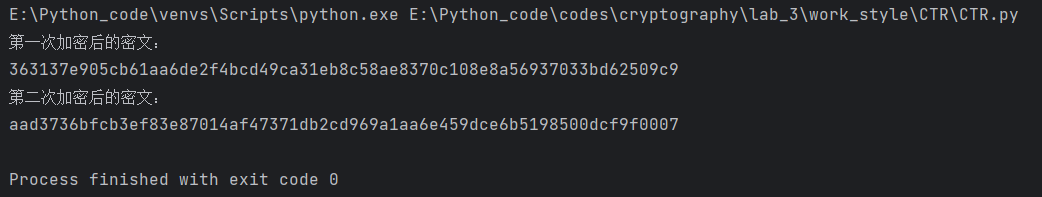
\includegraphics[width=13cm]{CTR_result_1.png}
                    \bottomcaption{\xiaowuhao{CTR相同明文加密两次结果}}
                \end{figure}
                通过观察发现,两次加密得到的结果不相同,所以CTR能够掩盖明文中的数据模式\par

        \subsubsection{各工作模式是否具有加密错误传播无界特性}
                选择第一次加密的明文为0001000101a198afda781734861535660001000101\\
                a198afda78173486153566aaa
                第二次加密的明文将第一位的0改为a然后进行加密,观察两次加密得出的密文进行判断\par
\newpage
            (1)ECB\par
                运行结果如下图所示
                \begin{figure}[H]
                    \centering
                    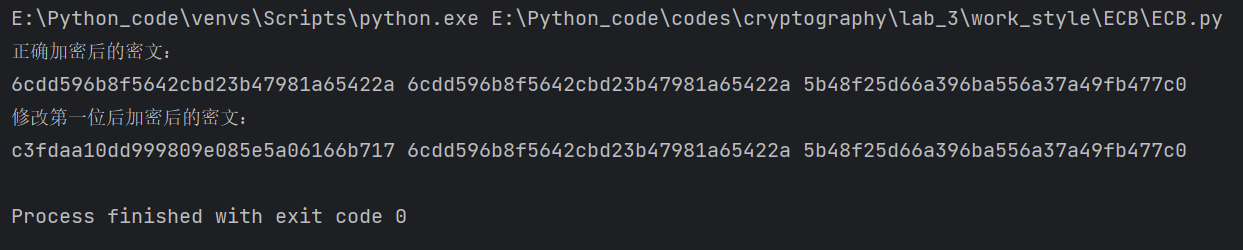
\includegraphics[width=13cm]{ECB_result_2.png}
                    \bottomcaption{\xiaowuhao{ECB修改一位明文两次加密结果}}
                \end{figure}
                通过观察发现,第一个分组的结果全体出现错误,但是影响范围只涉及到第一个分组,其他分组并未受到干扰,
                所以ECB工作模式具有加密错误传播有界的特性\par

            (2)MCBC\par
                运行结果如下图所示
                \begin{figure}[H]
                    \centering
                    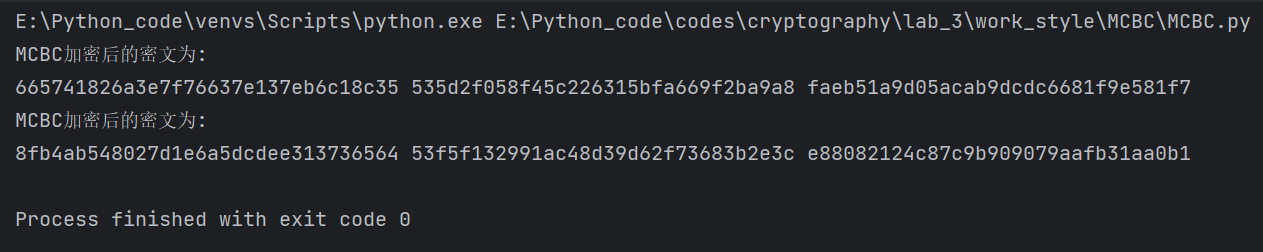
\includegraphics[width=13cm]{MCBC_result_2.png}
                    \bottomcaption{\xiaowuhao{MCBC修改一位明文两次加密结果}}
                \end{figure}
                通过观察发现,所有分组的加密结果均出现了错误,由此可见MCBC具有加密传播的无界性\par

            (3)CBC\par
                运行结果如下图所示
                \begin{figure}[H]
                    \centering
                    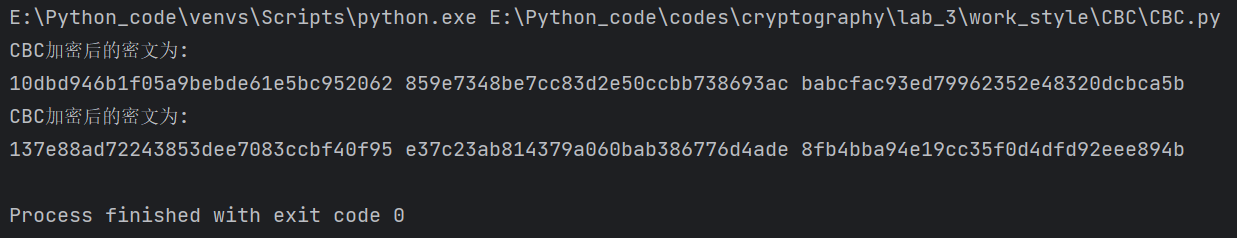
\includegraphics[width=13cm]{CBC_result_2.png}
                    \bottomcaption{\xiaowuhao{CBC修改一位明文两次加密结果}}
                \end{figure}
                通过观察发现,所有分组的加密结果均出现了错误,由此可见CBC具有加密传播的无界性\par
                
            (4)OFB\par
                运行结果如下图所示
                \begin{figure}[H]
                    \centering
                    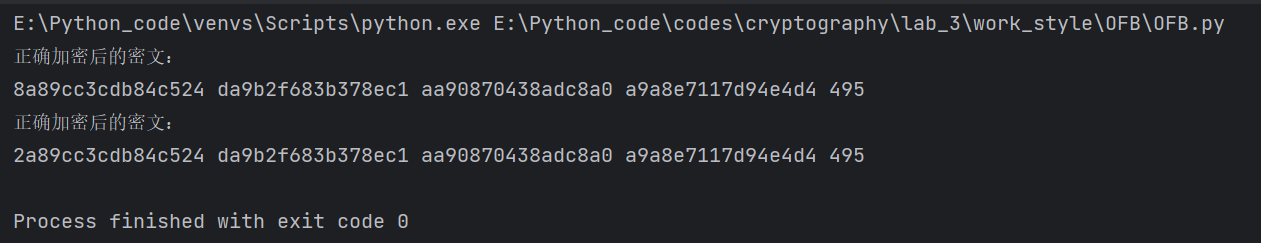
\includegraphics[width=13cm]{OFB_result_2.png}
                    \bottomcaption{\xiaowuhao{OFB修改一位明文两次加密结果}}
                \end{figure}
                通过观察发现,第一个分组的结果全体出现错误,但是影响范围只涉及到第一个分组,其他分组并未受到干扰,
                所以OFB工作模式具有加密错误传播有界的特性\par

            (5)CFB\par
                运行结果如下图所示
                \begin{figure}[H]
                    \centering
                    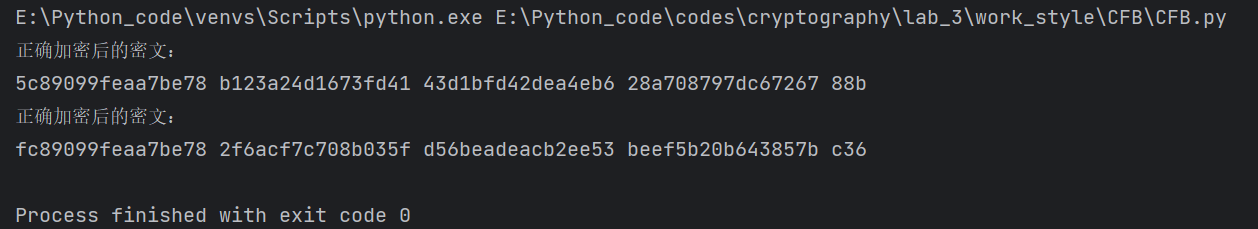
\includegraphics[width=13cm]{CFB_result_2.png}
                    \bottomcaption{\xiaowuhao{CFB修改一位明文两次加密结果}}
                \end{figure}
                通过观察发现,所有分组的加密结果均出现了错误,由此可见CFB具有加密传播的无界性\par
\newpage
            (6)XCBC\par
                运行结果如下图所示
                \begin{figure}[H]
                    \centering
                    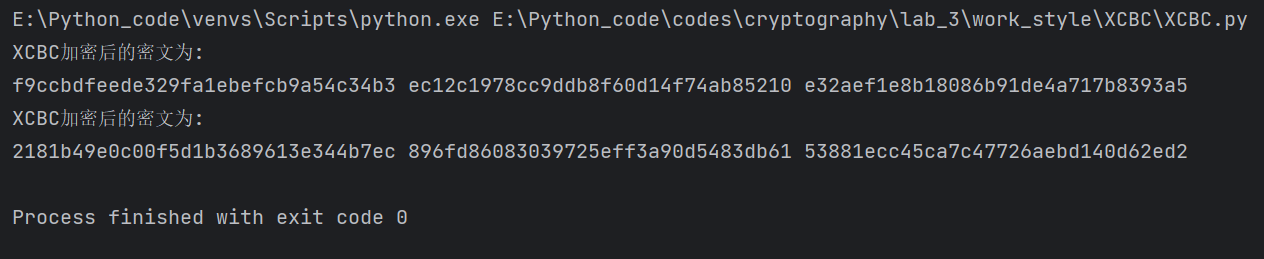
\includegraphics[width=13cm]{XCBC_result_2.png}
                    \bottomcaption{\xiaowuhao{XCBC修改一位明文两次加密结果}}
                \end{figure}
                通过观察发现,所有分组的加密结果均出现了错误,由此可见XCBC具有加密传播的无界性\par

            (7)CTR\par
                运行结果如下图所示
                \begin{figure}[H]
                    \centering
                    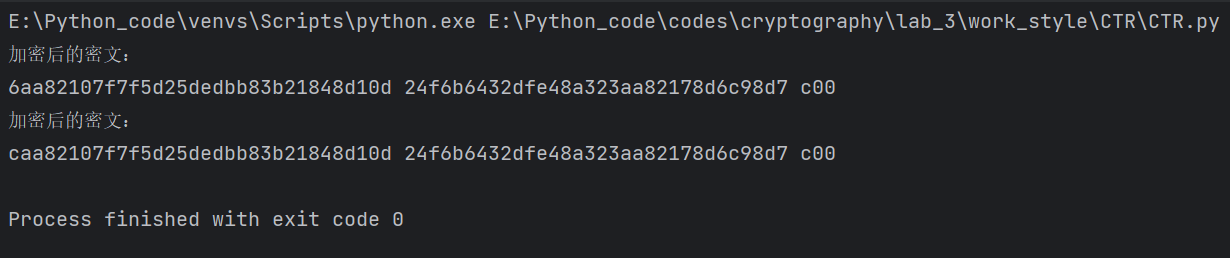
\includegraphics[width=13cm]{CTR_result_2.png}
                    \bottomcaption{\xiaowuhao{CTR修改一位明文两次加密结果}}
                \end{figure}
                通过观察发现,第一个分组的结果全体出现错误,但是影响范围只涉及到第一个分组,其他分组并未受到干扰,
                所以CTR工作模式具有加密错误传播有界的特性\par
\newpage                
        \subsubsection{各工作模式是否具有解密错误传播无界特性}
            将每一次实验中加密后得到的密文的首位与‘1’进行异或操作,即对密文的第一个分块进行修改,
            查看修改后的解密结果与正常解密结果之间的差异\par
            (1)ECB\par
                运行后的结果如下图所示
                \begin{figure}[H]
                    \centering
                    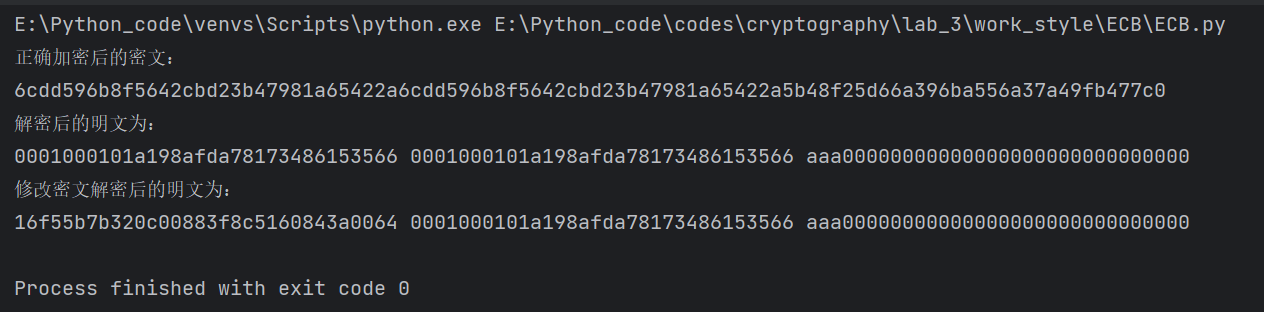
\includegraphics[width=13cm]{ECB_result_3.png}
                    \bottomcaption{\xiaowuhao{ECB修改一位密文后两次加密结果}}
                \end{figure}
                通过观察发现,在将第一块中的密文修改之后进行解密操作后得到的明文仅有第一个分组中出现错误,其余分组中
                解密出的明文与正常解密的明文相同,所以ECB具有解密错误传播有界的特性
                
            (2)MCBC\par
                运行后的结果如下图所示
                \begin{figure}[H]
                    \centering
                    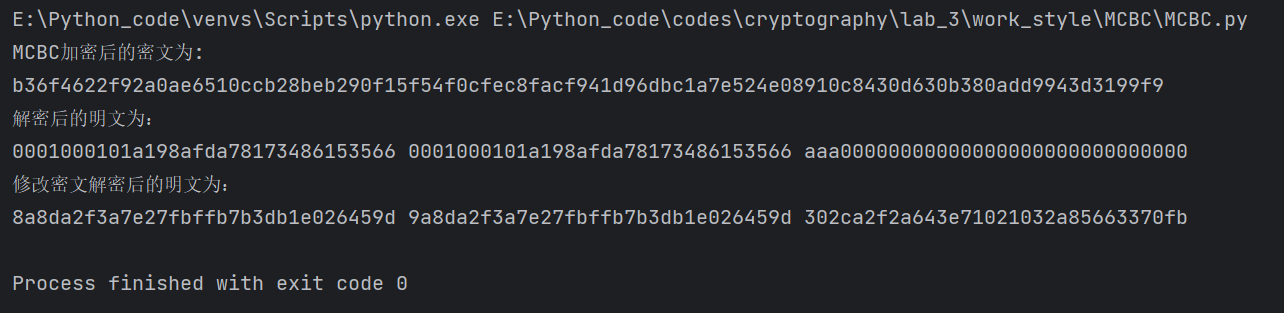
\includegraphics[width=13cm]{MCBC_result_3.png}
                    \bottomcaption{\xiaowuhao{MCBC修改一位密文后两次加密结果}}
                \end{figure}
                通过观察发现,在将第一块中的密文修改之后进行解密操作后得到的明文中的所有分组均出现了错误,
                所以MCBC具有解密错误传播无界的特性
\newpage
            (3)CBC\par
                运行后的结果如下图所示
                \begin{figure}[H]
                    \centering
                    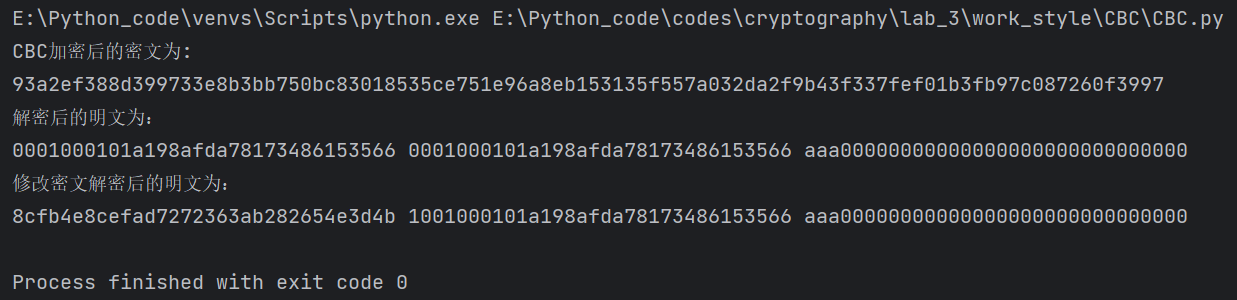
\includegraphics[width=13cm]{CBC_result_3.png}
                    \bottomcaption{\xiaowuhao{CBC修改一位密文后两次加密结果}}
                \end{figure}
                通过观察发现,在将第一块中的密文修改之后进行解密操作后得到的明文仅有第一个分组中出现错误以及第二个分组的首项出现错误,其余分组中
                解密出的明文与正常解密的明文相同,所以CBC具有解密错误传播有界的特性

            (4)OFB\par
                运行后的结果如下图所示
                \begin{figure}[H]
                    \centering
                    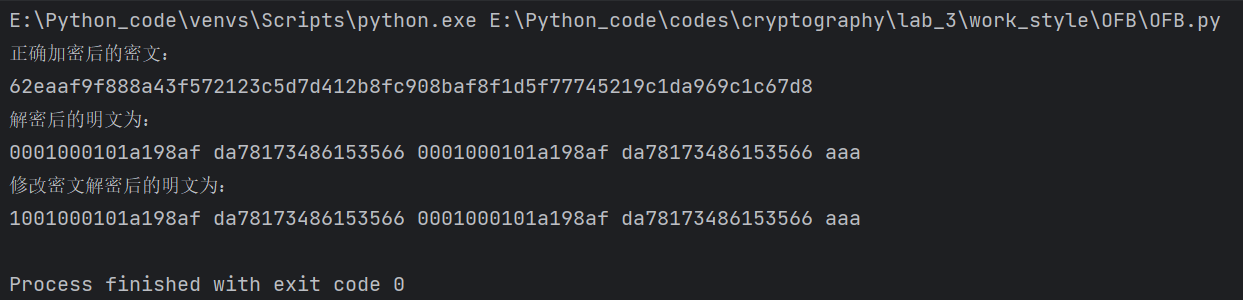
\includegraphics[width=13cm]{OFB_result_3.png}
                    \bottomcaption{\xiaowuhao{OFB修改一位密文后两次加密结果}}
                \end{figure}
                通过观察发现,在将第一块中的密文修改之后进行解密操作后得到的明文仅有第一个分组中出现错误,其余分组中
                解密出的明文与正常解密的明文相同,所以OFB具有解密错误传播有界的特性
\newpage
            (5)CFB\par
                运行后的结果如下图所示
                \begin{figure}[H]
                    \centering
                    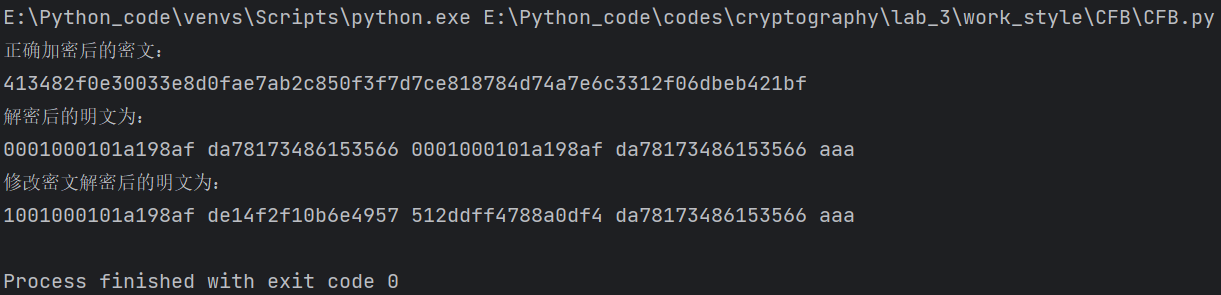
\includegraphics[width=13cm]{CFB_result_3.png}
                    \bottomcaption{\xiaowuhao{CFB修改一位密文后两次加密结果}}
                \end{figure}
                通过观察发现,在将第一块中的密文修改之后进行解密操作后得到的明文中的所有分组均出现了错误,
                所以CFB具有解密错误传播无界的特性

            (6)XCBC\par
                运行后的结果如下图所示
                \begin{figure}[H]
                    \centering
                    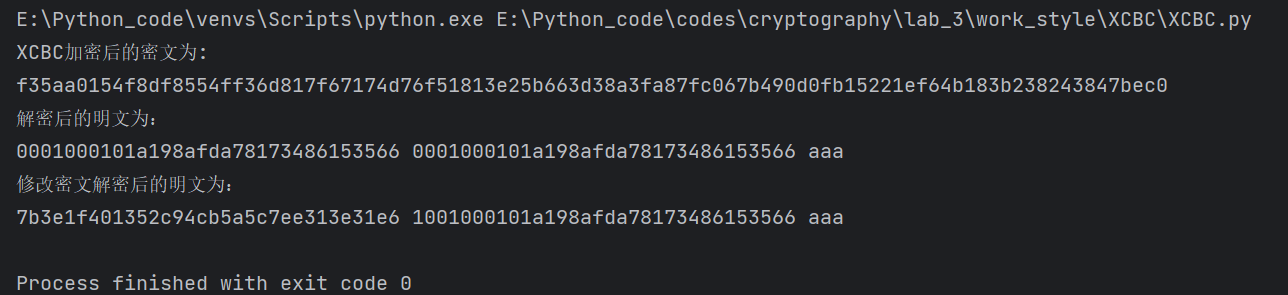
\includegraphics[width=13cm]{XCBC_result_3.png}
                    \bottomcaption{\xiaowuhao{XCBC修改一位密文后两次加密结果}}
                \end{figure}
                通过观察发现,在将第一块中的密文修改之后进行解密操作后得到的明文仅有第一个分组中出现错误以及第二个分组的首项出现错误,其余分组中
                解密出的明文与正常解密的明文相同,所以CBC具有解密错误传播有界的特性

            (7)CTR\par
                运行后的结果如下图所示
                \begin{figure}[H]
                    \centering
                    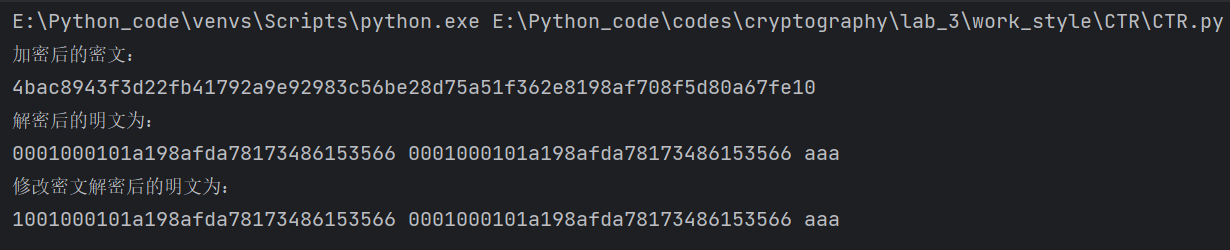
\includegraphics[width=13cm]{CTR_result_3.png}
                    \bottomcaption{\xiaowuhao{CTR修改一位密文后两次加密结果}}
                \end{figure}
                通过观察发现,在将第一块中的密文修改之后进行解密操作后得到的明文仅有第一个分组中出现错误,其余分组中
                解密出的明文与正常解密的明文相同,所以CTR具有解密错误传播有界的特性

        \subsubsection{不同的工作模式对于输入消息长度的要求}
            在7中不同的工作模式中只有ECB、CBC、明密文链接CBC模式要求输入的数据长度是密码分组长度的整数倍,其他工作模式均不对数据的长度做要求。

        \subsubsection{不同工作模式能否处理短块}
            在7中不同的工作模式中ECB、CBC、明密文链接CBC模式不具备天生的处理短块的能力,其余的工作模式均能够直接处理短块,无需额外的短块处理技术

        \subsubsection{不同工作模式是否改变消息长度}

            (1)ECB\par
                ECB加密的运行结果如下图所示
                \begin{figure}[H]
                    \centering
                    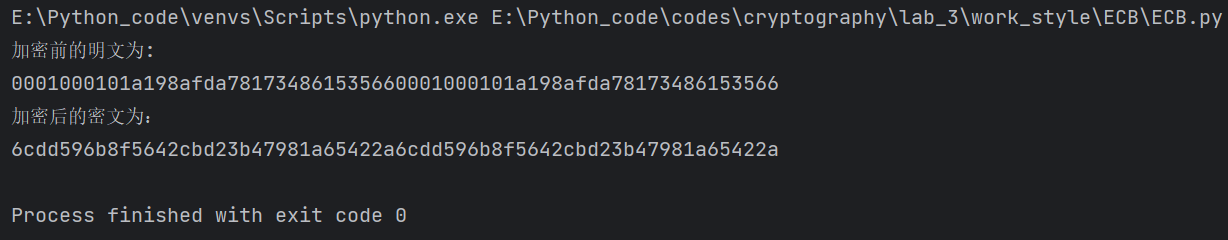
\includegraphics[width=13cm]{ECB_result_4.png}
                    \bottomcaption{\xiaowuhao{ECB加密结果}}
                \end{figure}
                通过观察可以发现ECB加密后的密文与加密前的明文位数相同,由此可见ECB工作模式不会改变信息的长度
\newpage
            (2)MCBC\par
                MCBC加密的运行结果如下图所示
                \begin{figure}[H]
                    \centering
                    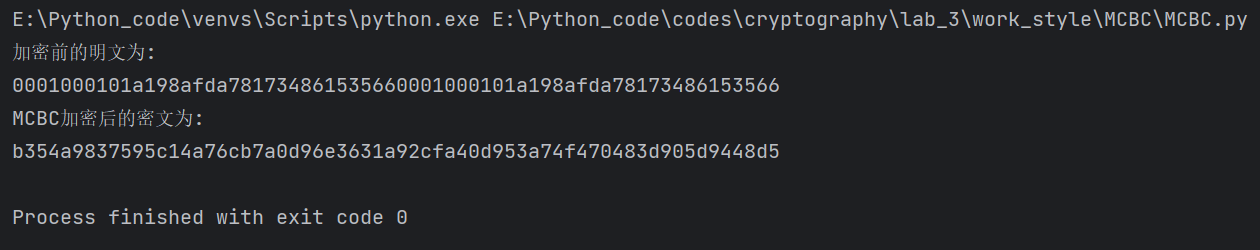
\includegraphics[width=13cm]{MCBC_result_4.png}
                    \bottomcaption{\xiaowuhao{MCBC加密结果}}
                \end{figure}
                通过观察可以发现MCBC加密后的密文与加密前的明文位数相同,但是因为输出的值还要包括初始向量IV所以
                密文的长度要长于明文,由此可见MCBC工作模式会改变信息的长度

            (3)CBC\par
                CBC加密的运行结果如下图所示
                \begin{figure}[H]
                    \centering
                    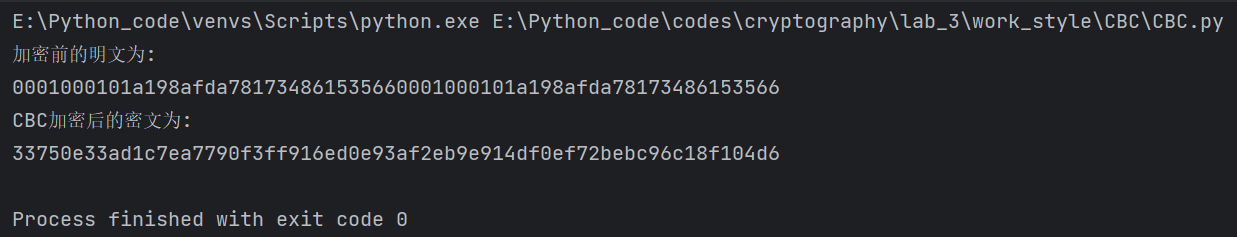
\includegraphics[width=13cm]{CBC_result_4.png}
                    \bottomcaption{\xiaowuhao{CBC加密结果}}
                \end{figure}
                通过观察可以发现CBC加密后的密文与加密前的明文位数相同,但是因为输出的值还要包括初始向量IV所以
                密文的长度要长于明文,由此可见CBC工作模式会改变信息的长度

            (4)OFB\par
                OFB加密的运行结果如下图所示
                \begin{figure}[H]
                    \centering
                    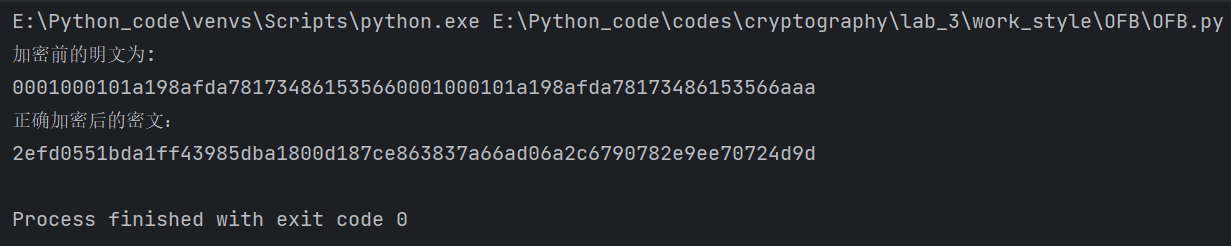
\includegraphics[width=13cm]{OFB_result_4.png}
                    \bottomcaption{\xiaowuhao{OFB加密结果}}
                \end{figure}
                通过观察可以发现OFB加密后的密文与加密前的明文位数相同,但是因为输出的值还要包括初始向量IV所以
                密文的长度要长于明文,由此可见OFB工作模式会改变信息的长度

            (5)CFB\par
                CFB加密的运行结果如下图所示
                \begin{figure}[H]
                    \centering
                    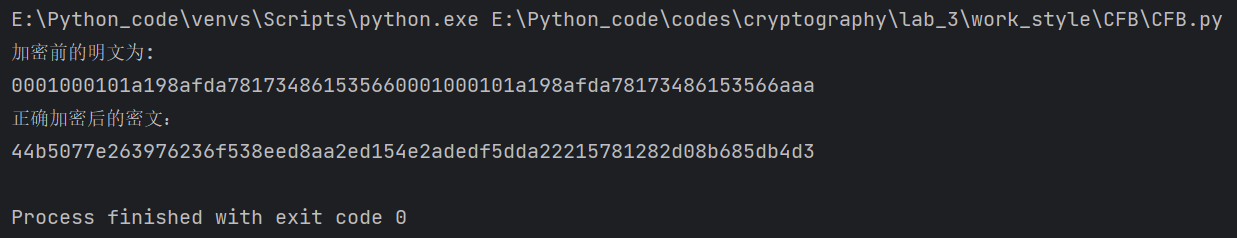
\includegraphics[width=13cm]{CFB_result_4.png}
                    \bottomcaption{\xiaowuhao{CFB加密结果}}
                \end{figure}
                通过观察可以发现CFB加密后的密文与加密前的明文位数相同,但是因为输出的值还要包括初始向量IV所以
                密文的长度要长于明文,由此可见CFB工作模式会改变信息的长度

            (6)XCBC\par
                XCBC加密的运行结果如下图所示
                \begin{figure}[H]
                    \centering
                    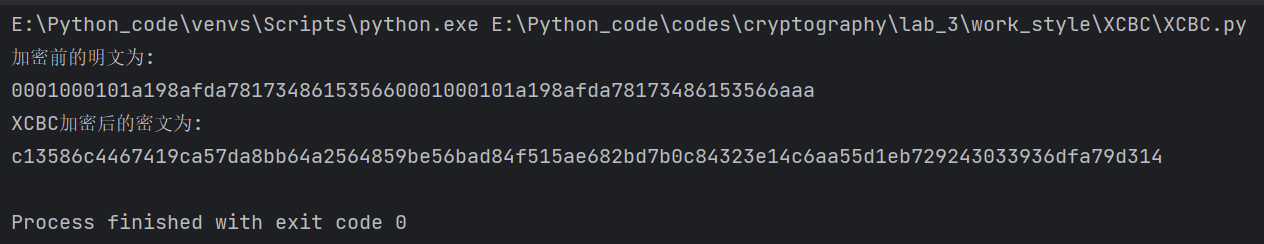
\includegraphics[width=13cm]{XCBC_result_4.png}
                    \bottomcaption{\xiaowuhao{XCBC加密结果}}
                \end{figure}
                通过观察可以发现XCBC加密后的密文与加密前的明文位数不同,加密后的密文位数增加,由此可见XCBC工作模式会改变信息的长度
\newpage
            (7)CTR\par
                CTR加密的运行结果如下图所示
                \begin{figure}[H]
                    \centering
                    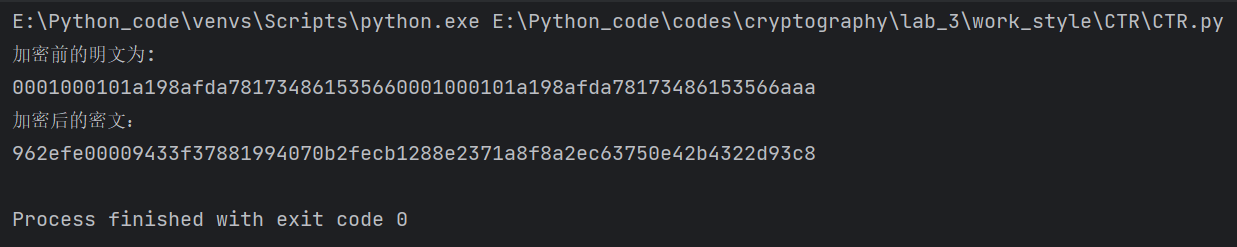
\includegraphics[width=13cm]{CTR_result_4.png}
                    \bottomcaption{\xiaowuhao{CTR加密结果}}
                \end{figure}
                通过观察可以发现CTR加密后的密文与加密前的明文位数相同,但是因为输出的值还要包括初始向量IV所以
                密文的长度要长于明文,由此可见CTR工作模式会改变信息的长度

        \subsubsection{不同的工作模式的执行效率}
            将每种工作模式程序中的提示输出注释掉之后统计每个工作模式的工作时间,并用工作时间除加密的比特数即可得知程序运行的效率\par
            在本次实验中使用如下程序统计每一种工作模式下的运行速率并输出。程序代码如下所示
            \lstinputlisting[caption={统计运行效率},captionpos=b]{E:/Python_code/codes/cryptography/lab_3/work_style/caculate_speed.py}
            程序运行的结果即各个工作模式的工作效率如下图所示
            \begin{figure}[H]
                \centering
                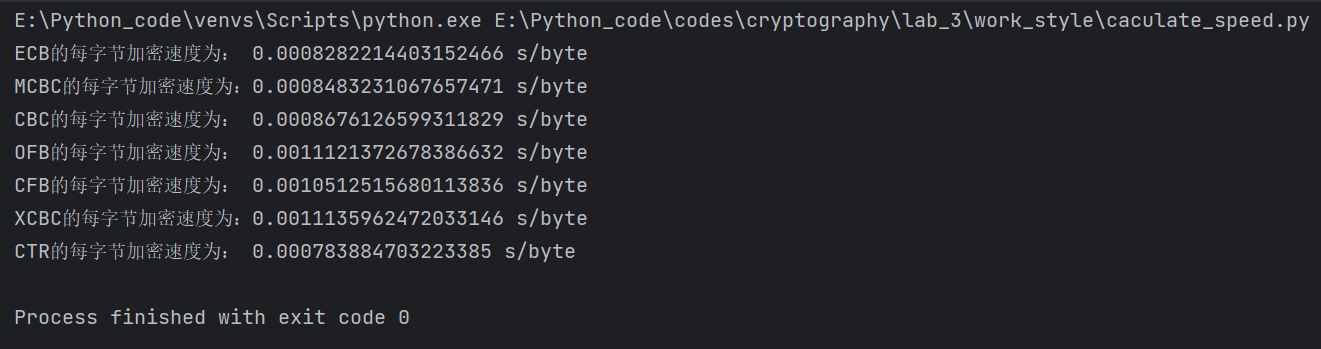
\includegraphics[width=13cm]{speed.png}
                \bottomcaption{\xiaowuhao{所有工作模式运行效率}}
            \end{figure}

    \subsection{短块处理技术的比较}
        \subsubsection{短块数据扩张}
            (1)短块填充法:\par
            填充法会导致数据扩张,因为它添加了额外的字节。数据块的最终大小将等于加密算法所需的固定块大小,即使原始数据较短。\par
            (2)序列密码加密法\par
            序列密码加密通常不会导致数据扩张。它生成的密文长度与原始数据长度相同,因为它是逐字节或逐位加密的。\par
            (3)密文挪用技术\par
            密文挪用技术通常不会导致数据扩张。它通过重新组织最后两个块的内容来确保输出数据与输入数据具有相同的长度,从而避免了填充带来的数据扩张。
        \subsubsection{安全性}

            (1)短块填充法\par
            这种填充方法本身并不增加明显的安全风险,因为添加的填充数据是固定和可预测的,不包含有关原始数据的敏感信息。
            然而,如果攻击者能够控制某些明文块并分析响应的密文变化,他们可能能够得出一些关于填充过程或加密算法的信息。
            但这种方法的安全性主要依赖于底层加密算法的强度。\par

            (2)序列密码加密法\par
            这种方法的安全性较高,因为它依赖于已加密的数据块,该数据块应该是难以预测和无法控制的。
            由于每个块的加密依赖于前一个块的密文,这为加密过程提供了额外的复杂性。在选择明文攻击中,
            即使攻击者可以选择明文块,他们也无法直接控制或预测用于加密的“密钥流”,这使得攻击变得困难。\par

            (3)密文挪用技术\par
            密文挪用技术不会增加额外的安全风险,因为它只是对最后两个块进行重新安排,而不是改变加密算法本身。
            它的目的是避免填充带来的潜在风险,同时保持数据长度不变。在选择明文攻击的情境下,
            这种方法并不提供额外的保护,但也不会降低现有的加密算法的安全性。\par

\section{实验结果与数据处理}

    \begin{table}[h!]
        \begin{center}
        \caption{各工作模式特点}
        \begin{tabular}{l|c|c|c|c|c|c|c} % <-- 8 columns
            \textbf{工作模式} & \textbf{ECB} & \textbf{明密文链接} & \textbf{CBC} & \textbf{OFB} & \textbf{CFB} & \textbf{XCBC} & \textbf{CTR} \\
            \hline
            能否掩盖数据模式    & 否    & 是    & 是    & 是    & 是    & 是    & 是 \\
            加密错误传播       & 有界   & 无界  & 无界  & 有界   & 无界  & 无界  & 有界 \\
            解密错误传播       &有界    & 无界  & 有界  & 有界   & 无界  & 有界  & 有界 \\
            是否改变消息长度   & 否     & 是    & 是    & 是    & 是    & 是    & 是 \\
            能否处理短块       & 否    & 否    &否      & 是    & 是    & 是    & 是 \\
            执行速度(ms/byte) & 0.828 & 0.848 & 0.868 & 1.112 & 1.051 & 1.114 & 0.784 \\
        \end{tabular}
        \end{center}
    \end{table}

    \begin{table}[h!]
        \begin{center}
          \caption{各短块处理技术特点}
          \begin{tabular}{l|c|c|c} % <-- 4 columns
            \textbf{短块处理方式} & \textbf{填充} & \textbf{序列密码加密} & \textbf{密文挪用} \\
            \hline
            短块数据扩张 & 会 & 否 & 否 \\
            实现难度     & 低 & 中 & 高 \\
            安全性      & 依赖加密算法 & 中 & 高 \\
          \end{tabular}
        \end{center}
    \end{table}
      
\section{分析与讨论}
    在这次的实验中,我深入探索了分组密码的各种工作模式,包括ECB(电子密码本模式)、CBC(密码块链接模式)、
    OFB(输出反馈模式)、CFB(密码反馈模式)和CTR(计数器模式),以及分组密码的短块加密技术。
    通过这个实验,我不仅提高了自己的理论知识,还获得了宝贵的实践经验,尤其是在处理任意长度输入数据的加密和解密方面。\par
    在实验中,我特别注意了短块加密技术的应用。通过使用填充法、序列密码加密法和密文挪用技术,
    我成功地对不满一个完整块的数据进行了有效处理。这些技术的实际应用不仅增强了我的编程技能,也加深了我对于这些概念的理解。\par
    利用这些工作模式和技术,我成功实现了对任意长度输入的加密和解密。这个过程不仅考验了我的理论知识,也锻炼了我的编程能力。
    我学会了如何根据不同的应用场景选择最合适的加密模式,并理解了在安全性和效率之间取得平衡的重要性。

\section{教师评语}

\end{document}
